% Options for packages loaded elsewhere
\PassOptionsToPackage{unicode}{hyperref}
\PassOptionsToPackage{hyphens}{url}
\PassOptionsToPackage{dvipsnames,svgnames,x11names}{xcolor}
%
\documentclass[
  letterpaper,
  DIV=11,
  numbers=noendperiod]{scrartcl}

\usepackage{amsmath,amssymb}
\usepackage{iftex}
\ifPDFTeX
  \usepackage[T1]{fontenc}
  \usepackage[utf8]{inputenc}
  \usepackage{textcomp} % provide euro and other symbols
\else % if luatex or xetex
  \usepackage{unicode-math}
  \defaultfontfeatures{Scale=MatchLowercase}
  \defaultfontfeatures[\rmfamily]{Ligatures=TeX,Scale=1}
\fi
\usepackage{lmodern}
\ifPDFTeX\else  
    % xetex/luatex font selection
\fi
% Use upquote if available, for straight quotes in verbatim environments
\IfFileExists{upquote.sty}{\usepackage{upquote}}{}
\IfFileExists{microtype.sty}{% use microtype if available
  \usepackage[]{microtype}
  \UseMicrotypeSet[protrusion]{basicmath} % disable protrusion for tt fonts
}{}
\makeatletter
\@ifundefined{KOMAClassName}{% if non-KOMA class
  \IfFileExists{parskip.sty}{%
    \usepackage{parskip}
  }{% else
    \setlength{\parindent}{0pt}
    \setlength{\parskip}{6pt plus 2pt minus 1pt}}
}{% if KOMA class
  \KOMAoptions{parskip=half}}
\makeatother
\usepackage{xcolor}
\setlength{\emergencystretch}{3em} % prevent overfull lines
\setcounter{secnumdepth}{-\maxdimen} % remove section numbering
% Make \paragraph and \subparagraph free-standing
\ifx\paragraph\undefined\else
  \let\oldparagraph\paragraph
  \renewcommand{\paragraph}[1]{\oldparagraph{#1}\mbox{}}
\fi
\ifx\subparagraph\undefined\else
  \let\oldsubparagraph\subparagraph
  \renewcommand{\subparagraph}[1]{\oldsubparagraph{#1}\mbox{}}
\fi


\providecommand{\tightlist}{%
  \setlength{\itemsep}{0pt}\setlength{\parskip}{0pt}}\usepackage{longtable,booktabs,array}
\usepackage{calc} % for calculating minipage widths
% Correct order of tables after \paragraph or \subparagraph
\usepackage{etoolbox}
\makeatletter
\patchcmd\longtable{\par}{\if@noskipsec\mbox{}\fi\par}{}{}
\makeatother
% Allow footnotes in longtable head/foot
\IfFileExists{footnotehyper.sty}{\usepackage{footnotehyper}}{\usepackage{footnote}}
\makesavenoteenv{longtable}
\usepackage{graphicx}
\makeatletter
\def\maxwidth{\ifdim\Gin@nat@width>\linewidth\linewidth\else\Gin@nat@width\fi}
\def\maxheight{\ifdim\Gin@nat@height>\textheight\textheight\else\Gin@nat@height\fi}
\makeatother
% Scale images if necessary, so that they will not overflow the page
% margins by default, and it is still possible to overwrite the defaults
% using explicit options in \includegraphics[width, height, ...]{}
\setkeys{Gin}{width=\maxwidth,height=\maxheight,keepaspectratio}
% Set default figure placement to htbp
\makeatletter
\def\fps@figure{htbp}
\makeatother

\KOMAoption{captions}{tableheading}
\makeatletter
\makeatother
\makeatletter
\makeatother
\makeatletter
\@ifpackageloaded{caption}{}{\usepackage{caption}}
\AtBeginDocument{%
\ifdefined\contentsname
  \renewcommand*\contentsname{Table of contents}
\else
  \newcommand\contentsname{Table of contents}
\fi
\ifdefined\listfigurename
  \renewcommand*\listfigurename{List of Figures}
\else
  \newcommand\listfigurename{List of Figures}
\fi
\ifdefined\listtablename
  \renewcommand*\listtablename{List of Tables}
\else
  \newcommand\listtablename{List of Tables}
\fi
\ifdefined\figurename
  \renewcommand*\figurename{Figure}
\else
  \newcommand\figurename{Figure}
\fi
\ifdefined\tablename
  \renewcommand*\tablename{Table}
\else
  \newcommand\tablename{Table}
\fi
}
\@ifpackageloaded{float}{}{\usepackage{float}}
\floatstyle{ruled}
\@ifundefined{c@chapter}{\newfloat{codelisting}{h}{lop}}{\newfloat{codelisting}{h}{lop}[chapter]}
\floatname{codelisting}{Listing}
\newcommand*\listoflistings{\listof{codelisting}{List of Listings}}
\makeatother
\makeatletter
\@ifpackageloaded{caption}{}{\usepackage{caption}}
\@ifpackageloaded{subcaption}{}{\usepackage{subcaption}}
\makeatother
\makeatletter
\@ifpackageloaded{tcolorbox}{}{\usepackage[skins,breakable]{tcolorbox}}
\makeatother
\makeatletter
\@ifundefined{shadecolor}{\definecolor{shadecolor}{rgb}{.97, .97, .97}}
\makeatother
\makeatletter
\makeatother
\makeatletter
\makeatother
\ifLuaTeX
  \usepackage{selnolig}  % disable illegal ligatures
\fi
\IfFileExists{bookmark.sty}{\usepackage{bookmark}}{\usepackage{hyperref}}
\IfFileExists{xurl.sty}{\usepackage{xurl}}{} % add URL line breaks if available
\urlstyle{same} % disable monospaced font for URLs
\hypersetup{
  pdftitle={Comparing Health Events in Populations: A Framework for Analysis},
  pdfauthor={Eric Delmelle},
  colorlinks=true,
  linkcolor={blue},
  filecolor={Maroon},
  citecolor={Blue},
  urlcolor={Blue},
  pdfcreator={LaTeX via pandoc}}

\title{Comparing Health Events in Populations: A Framework for Analysis}
\author{Eric Delmelle}
\date{}

\begin{document}
\maketitle
\ifdefined\Shaded\renewenvironment{Shaded}{\begin{tcolorbox}[breakable, interior hidden, enhanced, boxrule=0pt, sharp corners, borderline west={3pt}{0pt}{shadecolor}, frame hidden]}{\end{tcolorbox}}\fi

\begin{figure}

{\centering 
\includegraphics[width=0.7\textwidth,height=\textheight]{week2_files/imgs/banner.jpg}

}

\end{figure}

\begin{center}\rule{0.5\linewidth}{0.5pt}\end{center}

\hypertarget{introduction}{%
\subsection{\texorpdfstring{{\textbf{Introduction}}}{Introduction}}\label{introduction}}

\begin{itemize}
\tightlist
\item
  \textbf{Definition of Health Events}: Disease outbreaks, chronic
  conditions, injuries, and health behaviors.
\item
  \textbf{Importance of Comparisons}: Understanding disparities,
  identifying risk factors, guiding public health interventions.
\item
  \textbf{Key Concepts}: Population health, epidemiology, and
  biostatistics.
\end{itemize}

\begin{center}\rule{0.5\linewidth}{0.5pt}\end{center}

\hypertarget{objectives-of-population-health}{%
\subsection{\texorpdfstring{{\textbf{Objectives of Population
Health}}}{Objectives of Population Health}}\label{objectives-of-population-health}}

\hypertarget{four-key-objectives}{%
\subsubsection{\texorpdfstring{{\textbf{Four Key
Objectives}}:}{Four Key Objectives:}}\label{four-key-objectives}}

\begin{enumerate}
\def\labelenumi{\arabic{enumi}.}
\tightlist
\item
  \textbf{Describe}: Understand population-level health outcomes.\\
\item
  \textbf{Explain}: Identify determinants and drivers of health
  outcomes.\\
\item
  \textbf{Predict}: Anticipate future health trends and patterns.\\
\item
  \textbf{Control}: Implement interventions to improve outcomes.
\end{enumerate}

\begin{center}\rule{0.5\linewidth}{0.5pt}\end{center}

\hypertarget{historical-context}{%
\subsection{\texorpdfstring{{\textbf{Historical
Context}}}{Historical Context}}\label{historical-context}}

\hypertarget{key-figures}{%
\subsubsection{\texorpdfstring{{\textbf{Key
Figures}}:}{Key Figures:}}\label{key-figures}}

\begin{itemize}
\tightlist
\item
  \textbf{John Snow}: Cholera outbreak mapping.\\
\item
  \textbf{Ignaz Semmelweis}: Importance of handwashing.\\
\item
  \textbf{Joseph Goldberger}: Nutritional causes of pellagra.
\end{itemize}

\begin{center}\rule{0.5\linewidth}{0.5pt}\end{center}

\hypertarget{type-of-comparisons}{%
\subsection{\texorpdfstring{{\textbf{Type of
Comparisons}}}{Type of Comparisons}}\label{type-of-comparisons}}

\hypertarget{time-based}{%
\subsubsection{\texorpdfstring{{\textbf{Time-Based}}}{Time-Based}}\label{time-based}}

\begin{figure}

{\centering 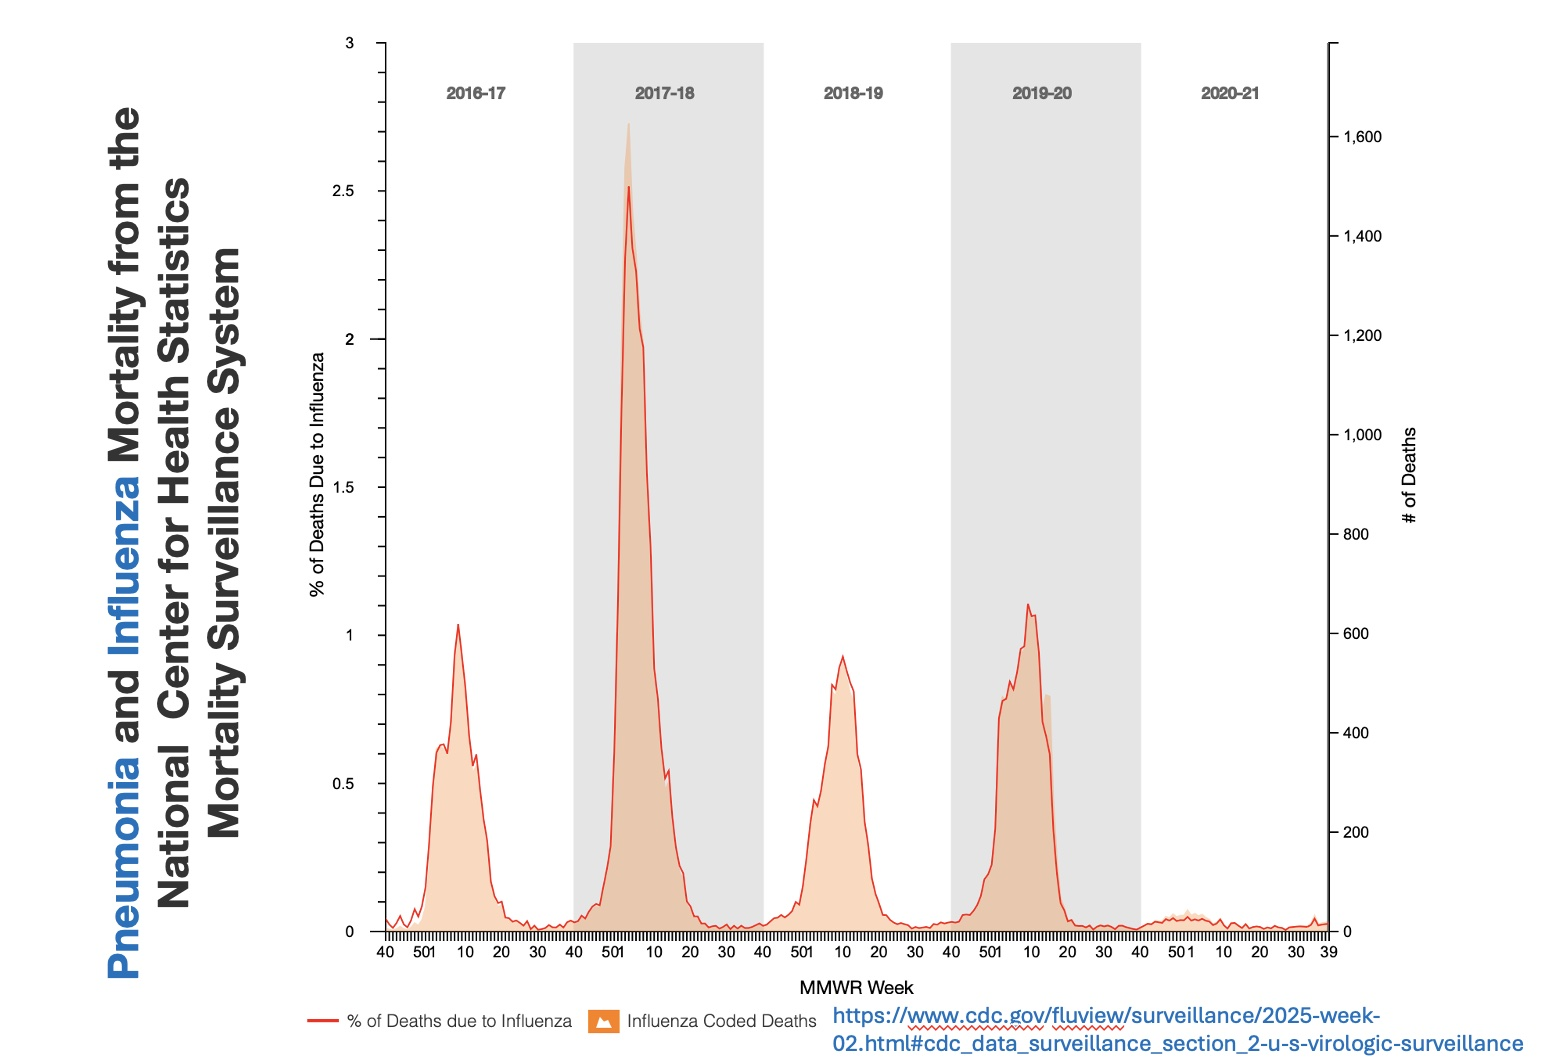
\includegraphics[width=0.7\textwidth,height=\textheight]{week2_files/imgs/timeBased.jpg}

}

\end{figure}

\hypertarget{key-metrics}{%
\paragraph{Key Metrics:}\label{key-metrics}}

\begin{itemize}
\tightlist
\item
  \textbf{Incidence}: New cases over time.
\item
  \textbf{Prevalence}: Existing cases at a given time.
\end{itemize}

\begin{center}\rule{0.5\linewidth}{0.5pt}\end{center}

\hypertarget{place-based}{%
\subsubsection{\texorpdfstring{{\textbf{Place-Based}}}{Place-Based}}\label{place-based}}

\begin{figure}

{\centering 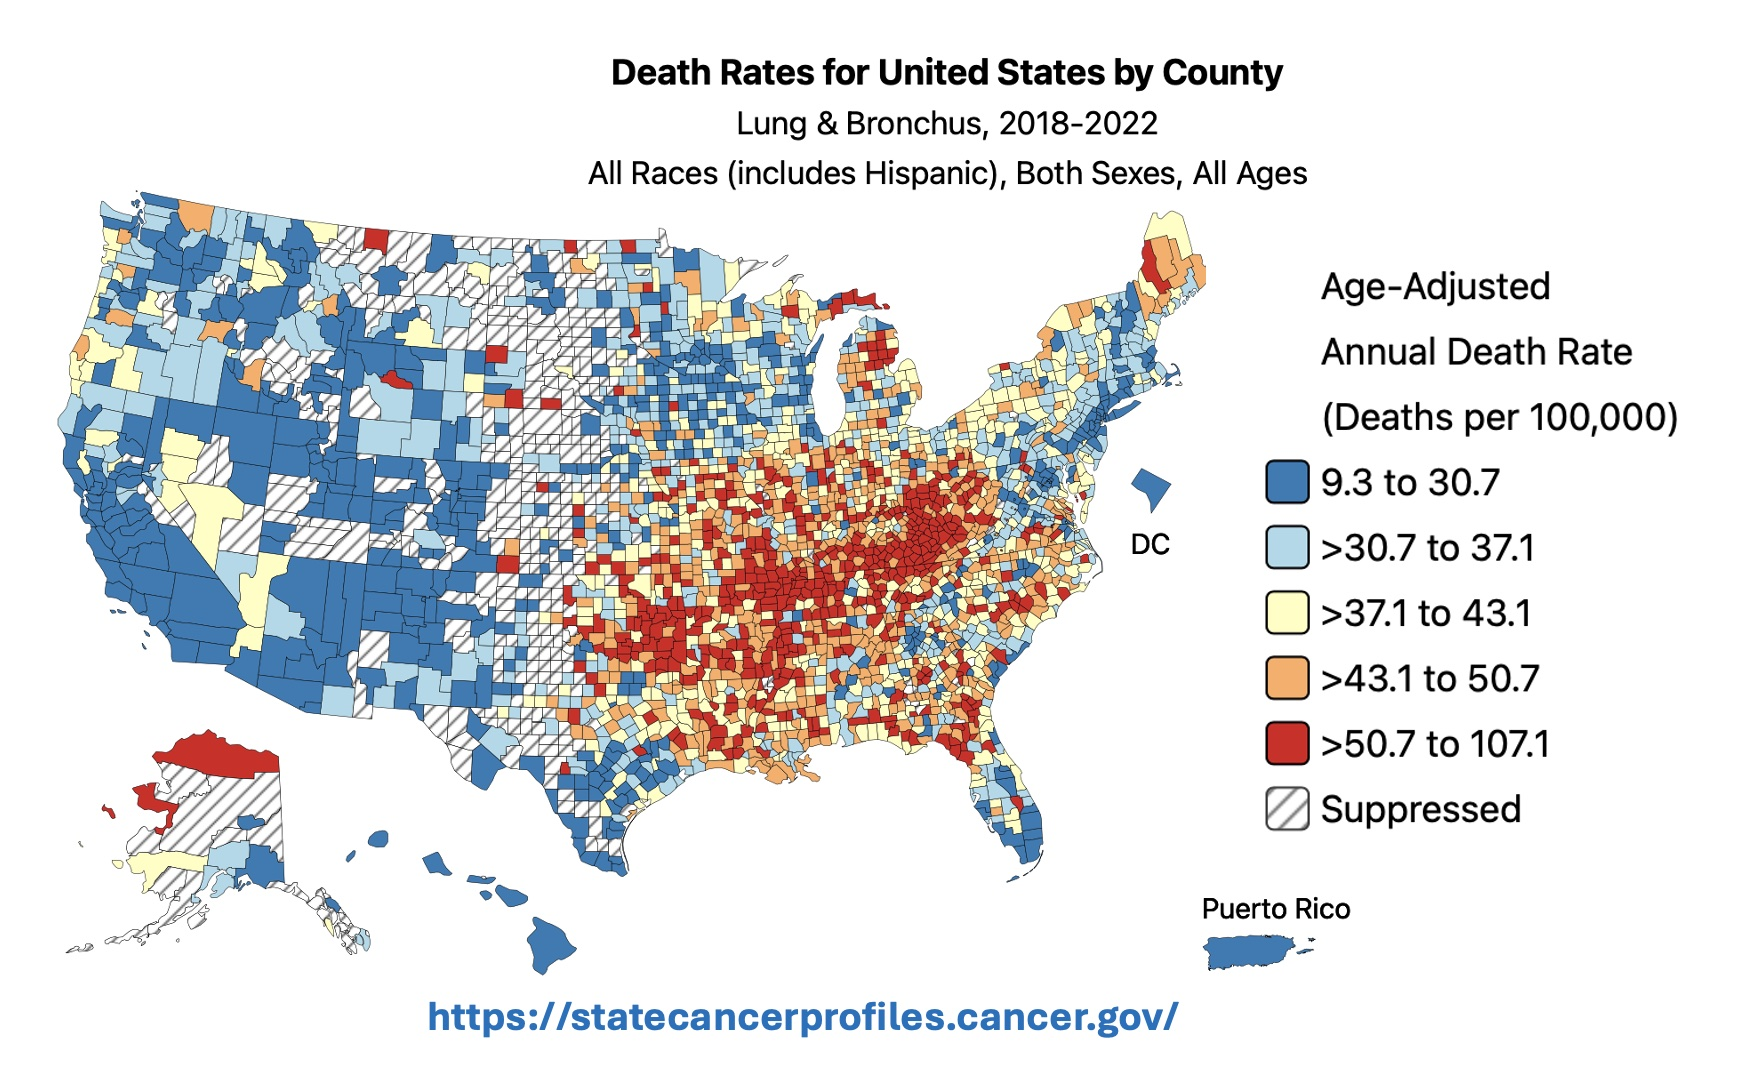
\includegraphics[width=0.7\textwidth,height=\textheight]{week2_files/imgs/placeBased.jpg}

}

\end{figure}

\hypertarget{example}{%
\paragraph{Example:}\label{example}}

\begin{itemize}
\tightlist
\item
  \textbf{Urban vs.~Rural Heart Disease Mortality}:

  \begin{itemize}
  \tightlist
  \item
    Urban: 50 per 100,000.\\
  \item
    Rural: 75 per 100,000.
  \end{itemize}
\end{itemize}

\begin{center}\rule{0.5\linewidth}{0.5pt}\end{center}

\hypertarget{group-based}{%
\subsubsection{\texorpdfstring{{\textbf{Group-Based}}}{Group-Based}}\label{group-based}}

\hypertarget{example-1}{%
\paragraph{Example:}\label{example-1}}

\begin{itemize}
\tightlist
\item
  Health disparities by race, age, and income.
  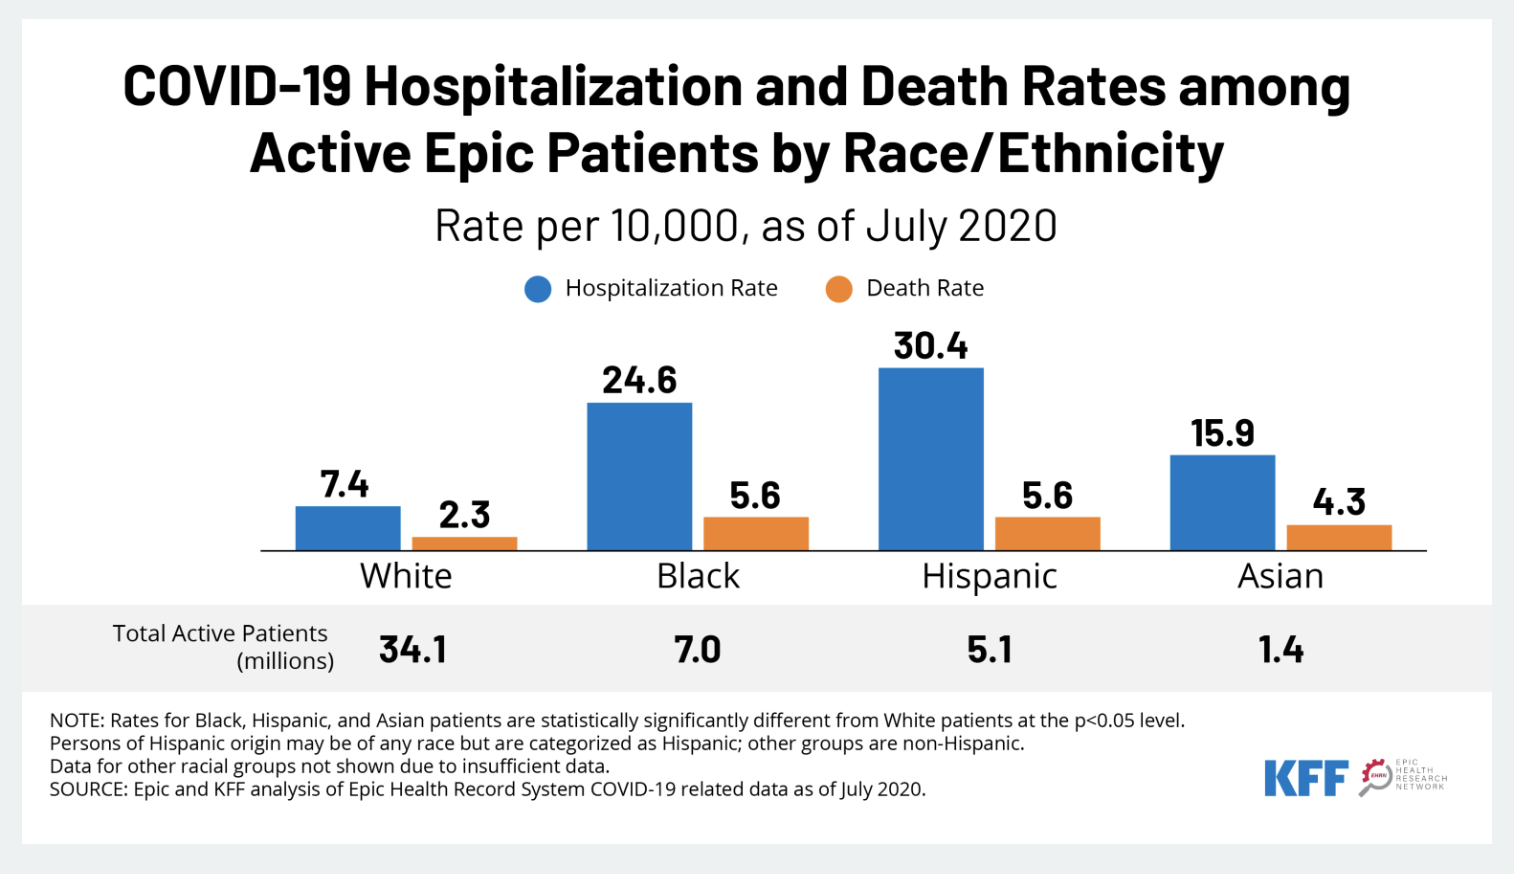
\includegraphics[width=0.7\textwidth,height=\textheight]{week2_files/imgs/covid19.png}
\end{itemize}

\begin{center}\rule{0.5\linewidth}{0.5pt}\end{center}

\hypertarget{event-based}{%
\subsubsection{\texorpdfstring{{\textbf{Event-Based}}}{Event-Based}}\label{event-based}}

\hypertarget{key-concept}{%
\paragraph{Key Concept:}\label{key-concept}}

\begin{itemize}
\tightlist
\item
  Natural experiments: Before vs.~after policy changes or interventions.
\end{itemize}

\begin{figure}

{\centering 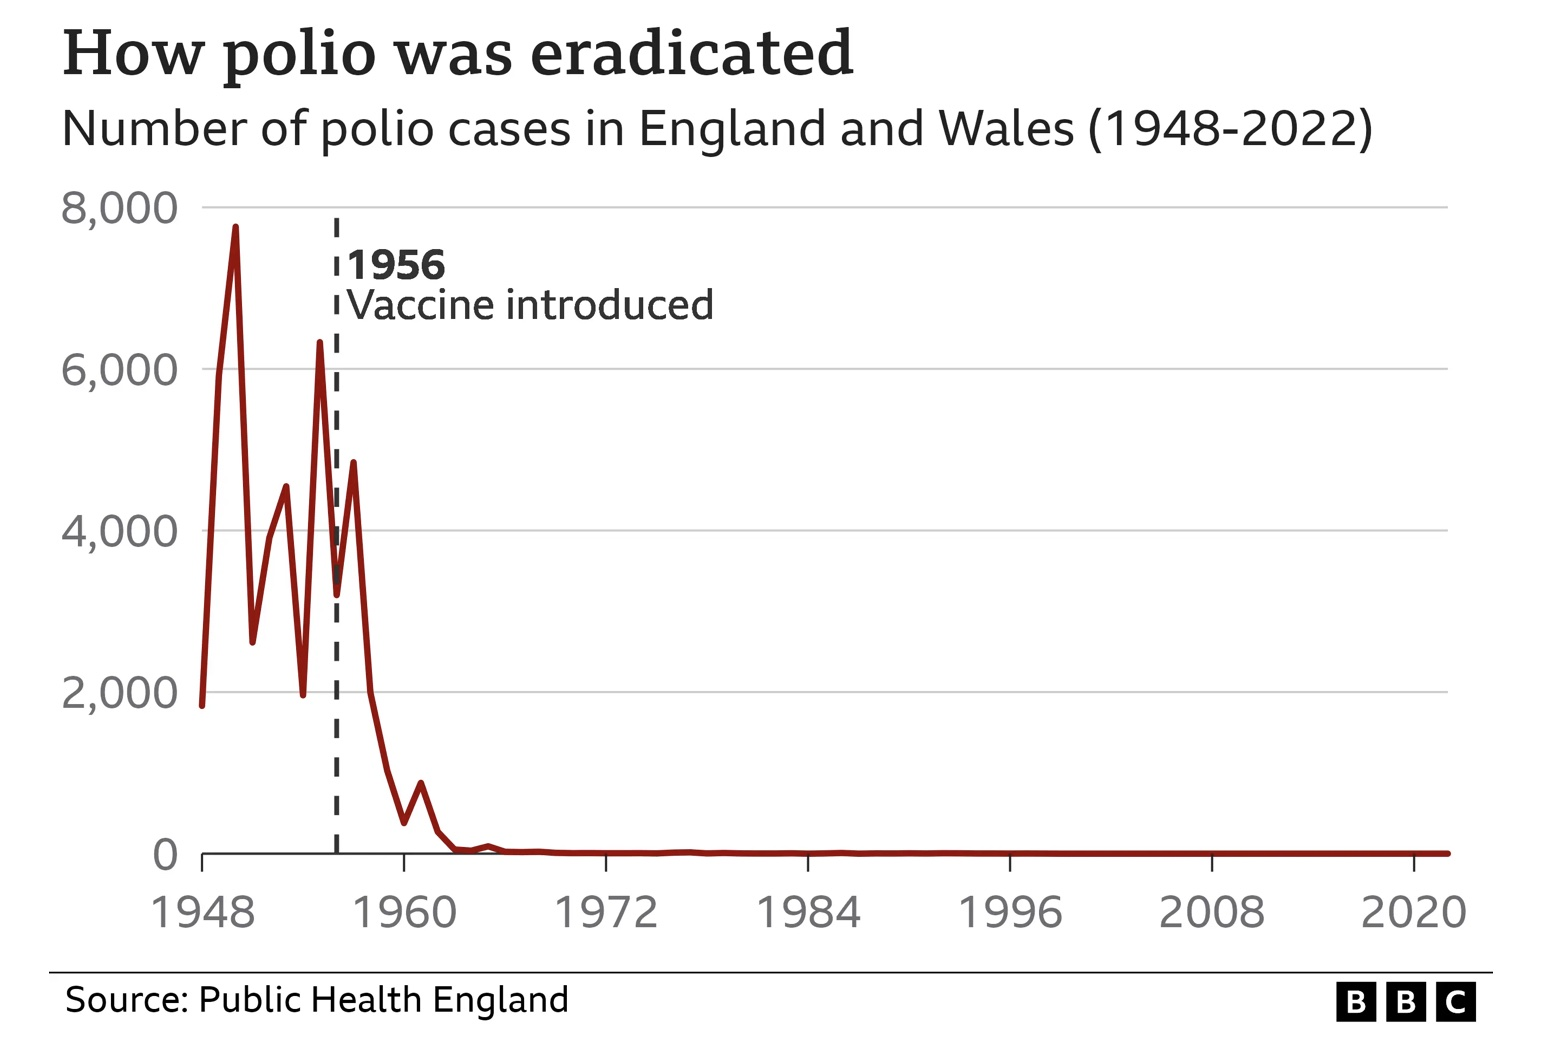
\includegraphics[width=0.7\textwidth,height=\textheight]{week2_files/imgs/polio.jpg}

}

\end{figure}

\begin{center}\rule{0.5\linewidth}{0.5pt}\end{center}

\hypertarget{additional-event-based-example}{%
\subsubsection{\texorpdfstring{{\textbf{Additional Event-Based
Example}}}{Additional Event-Based Example}}\label{additional-event-based-example}}

\begin{figure}

{\centering 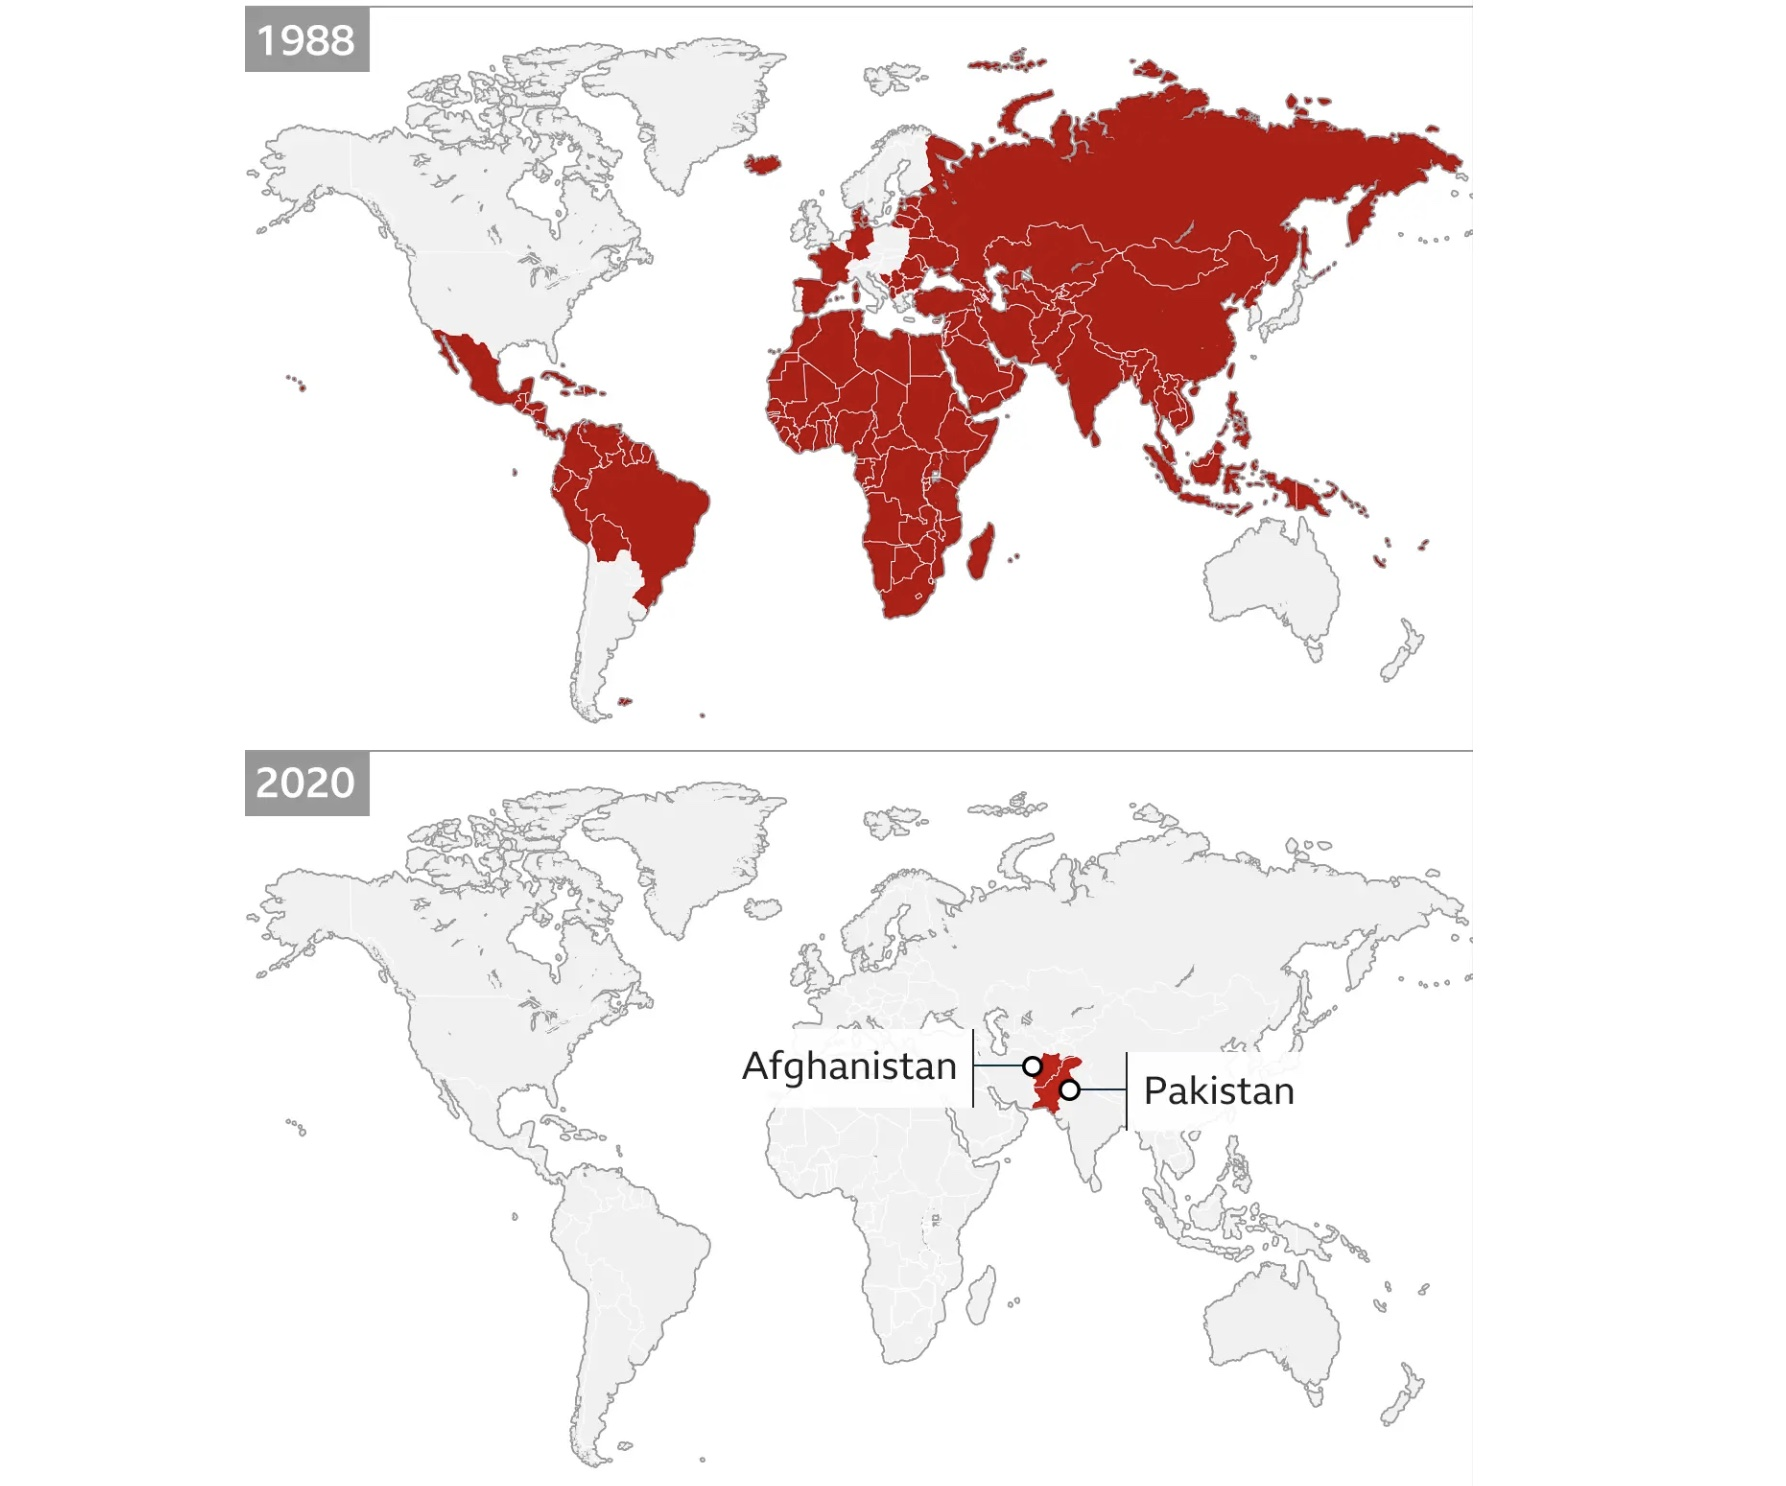
\includegraphics[width=0.7\textwidth,height=\textheight]{week2_files/imgs/polio2.jpg}

}

\end{figure}

\begin{center}\rule{0.5\linewidth}{0.5pt}\end{center}

\hypertarget{measures-of-comparison}{%
\subsection{\texorpdfstring{{\textbf{Measures of
Comparison}}}{Measures of Comparison}}\label{measures-of-comparison}}

\hypertarget{key-metrics-1}{%
\subsubsection{\texorpdfstring{{\textbf{Key
Metrics}}:}{Key Metrics:}}\label{key-metrics-1}}

\begin{itemize}
\tightlist
\item
  \textbf{Age-Standardized Rates}: Adjusted to eliminate age structure
  differences.
\item
  \textbf{Attributable Risk}: Measures the impact of specific risk
  factors on outcomes.
\end{itemize}

\begin{center}\rule{0.5\linewidth}{0.5pt}\end{center}

\hypertarget{levels-of-analysis}{%
\subsection{\texorpdfstring{{\textbf{Levels of
Analysis}}}{Levels of Analysis}}\label{levels-of-analysis}}

\hypertarget{frameworks}{%
\subsubsection{\texorpdfstring{{\textbf{Frameworks}}:}{Frameworks:}}\label{frameworks}}

\begin{itemize}
\tightlist
\item
  \textbf{Individual-Level}: Biostatistical and clinical trials.
\item
  \textbf{Population-Level}: Geographic and demographic patterns.
\end{itemize}

\begin{center}\rule{0.5\linewidth}{0.5pt}\end{center}

\hypertarget{determinants-of-health}{%
\subsection{\texorpdfstring{{\textbf{Determinants of
Health}}}{Determinants of Health}}\label{determinants-of-health}}

\hypertarget{categories}{%
\subsubsection{\texorpdfstring{{\textbf{Categories}}:}{Categories:}}\label{categories}}

\begin{enumerate}
\def\labelenumi{\arabic{enumi}.}
\tightlist
\item
  \textbf{Social and Economic Factors}
\item
  \textbf{Environmental Conditions}
\item
  \textbf{Behavioral and Genetic Influences}
\end{enumerate}

\begin{center}\rule{0.5\linewidth}{0.5pt}\end{center}

\hypertarget{challenges-in-comparisons}{%
\subsection{\texorpdfstring{{\textbf{Challenges in
Comparisons}}}{Challenges in Comparisons}}\label{challenges-in-comparisons}}

\hypertarget{key-challenges}{%
\subsubsection{\texorpdfstring{{\textbf{Key
Challenges}}:}{Key Challenges:}}\label{key-challenges}}

\begin{itemize}
\tightlist
\item
  \textbf{Data Quality}: Inaccuracies or incomplete datasets.\\
\item
  \textbf{Ethical Considerations}: Privacy and fair comparisons.
\end{itemize}

\begin{center}\rule{0.5\linewidth}{0.5pt}\end{center}

\hypertarget{population-vs.-community-health-assessments}{%
\subsection{\texorpdfstring{{\textbf{Population vs.~Community Health
Assessments}}}{Population vs.~Community Health Assessments}}\label{population-vs.-community-health-assessments}}

\hypertarget{key-differences}{%
\subsubsection{\texorpdfstring{{\textbf{Key
Differences}}:}{Key Differences:}}\label{key-differences}}

\begin{itemize}
\tightlist
\item
  \textbf{Community Health Assessments}:

  \begin{itemize}
  \tightlist
  \item
    Focus on local needs/resources.
  \item
    Qualitative methods (e.g., interviews).
  \end{itemize}
\item
  \textbf{Population Health Assessments}:

  \begin{itemize}
  \tightlist
  \item
    Broad, systemic focus.\\
  \item
    Quantitative data (e.g., chronic disease rates).
  \end{itemize}
\end{itemize}

\begin{center}\rule{0.5\linewidth}{0.5pt}\end{center}

\hypertarget{population-vs.-community-health-assessments-1}{%
\subsection{\texorpdfstring{{\textbf{Population vs.~Community Health
Assessments}}}{Population vs.~Community Health Assessments}}\label{population-vs.-community-health-assessments-1}}

\hypertarget{example-2}{%
\paragraph{Example:}\label{example-2}}

\begin{itemize}
\tightlist
\item
  Community: Identifying food deserts.\\
\item
  Population: Obesity prevalence across counties.
\end{itemize}

\begin{center}\rule{0.5\linewidth}{0.5pt}\end{center}

\hypertarget{policy-implications}{%
\subsection{\texorpdfstring{{\textbf{Policy
Implications}}}{Policy Implications}}\label{policy-implications}}

\hypertarget{using-comparisons-to-drive-change}{%
\subsubsection{\texorpdfstring{{\textbf{Using Comparisons to Drive
Change}}:}{Using Comparisons to Drive Change:}}\label{using-comparisons-to-drive-change}}

\begin{enumerate}
\def\labelenumi{\arabic{enumi}.}
\tightlist
\item
  \textbf{Set Priorities}: Identify at-risk groups (e.g., elderly,
  low-income communities).\\
\item
  \textbf{Develop Interventions}: Targeted programs (e.g., tobacco
  cessation).\\
\item
  \textbf{Advocate for Policy Change}: Use data for systemic reforms.
\end{enumerate}

\begin{center}\rule{0.5\linewidth}{0.5pt}\end{center}

\hypertarget{policy-implications-1}{%
\subsection{\texorpdfstring{{\textbf{Policy
Implications}}}{Policy Implications}}\label{policy-implications-1}}

\hypertarget{visual}{%
\paragraph{Visual:}\label{visual}}

\begin{figure}

{\centering 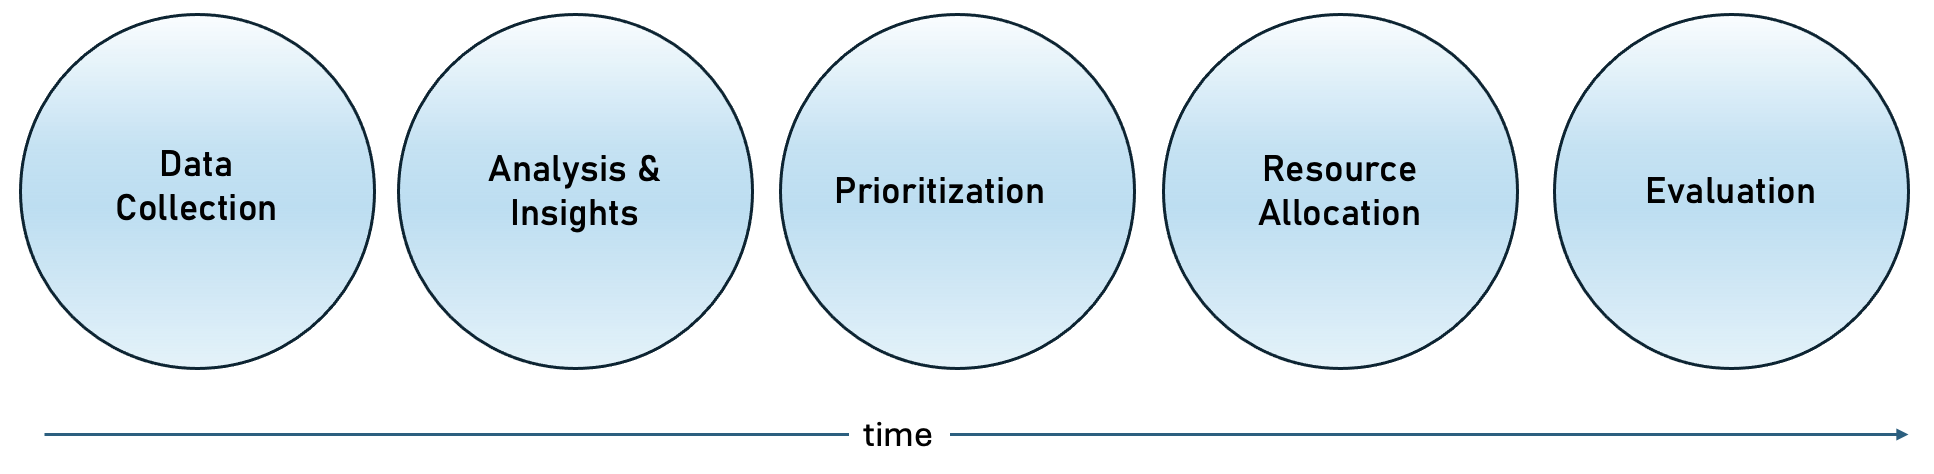
\includegraphics[width=0.8\textwidth,height=\textheight]{week2_files/imgs/dataDrivenComparison.png}

}

\end{figure}

\begin{center}\rule{0.5\linewidth}{0.5pt}\end{center}

\hypertarget{interactive-example}{%
\subsection{\texorpdfstring{{\textbf{Interactive
Example}}}{Interactive Example}}\label{interactive-example}}

\hypertarget{dataset-example}{%
\subsubsection{\texorpdfstring{{\textbf{Dataset
Example}}:}{Dataset Example:}}\label{dataset-example}}

\begin{longtable}[]{@{}lll@{}}
\toprule\noalign{}
Population & Cases & Rate (per 100,000) \\
\midrule\noalign{}
\endhead
\bottomrule\noalign{}
\endlastfoot
Urban & 200 & 50 \\
Rural & 300 & 75 \\
\end{longtable}

\hypertarget{prompt}{%
\paragraph{Prompt:}\label{prompt}}

\begin{itemize}
\tightlist
\item
  ``What does this suggest about resource allocation?''
\end{itemize}

\begin{center}\rule{0.5\linewidth}{0.5pt}\end{center}

\hypertarget{recap-and-transition}{%
\subsection{\texorpdfstring{{\textbf{Recap and
Transition}}}{Recap and Transition}}\label{recap-and-transition}}

\hypertarget{key-takeaways}{%
\subsubsection{\texorpdfstring{{\textbf{Key
Takeaways}}:}{Key Takeaways:}}\label{key-takeaways}}

\begin{itemize}
\tightlist
\item
  Importance of describing, explaining, predicting, and controlling
  health events.\\
\item
  Tools and methods to compare health outcomes.\\
\item
  Practical implications for population health strategies.
\end{itemize}

\hypertarget{next}{%
\paragraph{Next:}\label{next}}

\begin{itemize}
\tightlist
\item
  Group activity: Apply concepts to a real-world health disparity.
\end{itemize}

\begin{center}\rule{0.5\linewidth}{0.5pt}\end{center}

\hypertarget{group-activity-population-health-comparison}{%
\subsection{\texorpdfstring{{\textbf{Group Activity: Population Health
Comparison}}}{Group Activity: Population Health Comparison}}\label{group-activity-population-health-comparison}}

\hypertarget{objective}{%
\subsubsection{\texorpdfstring{{\textbf{Objective}}:}{Objective:}}\label{objective}}

Apply Chapter 1 metrics to analyze health disparities.

\hypertarget{instructions}{%
\subsubsection{\texorpdfstring{{\textbf{Instructions}}:}{Instructions:}}\label{instructions}}

\begin{enumerate}
\def\labelenumi{\arabic{enumi}.}
\tightlist
\item
  Form groups of 3--5.\\
\end{enumerate}

\begin{center}\rule{0.5\linewidth}{0.5pt}\end{center}

\hypertarget{instructions-1}{%
\subsubsection{\texorpdfstring{{\textbf{Instructions}}:}{Instructions:}}\label{instructions-1}}

\begin{enumerate}
\def\labelenumi{\arabic{enumi}.}
\setcounter{enumi}{1}
\tightlist
\item
  Analyze the provided dataset on coursesite

  \begin{itemize}
  \tightlist
  \item
    Calculate rates (e.g., incidence, prevalence).\\
  \item
    Identify disparities (e.g., geographic, demographic).\\
  \item
    Propose targeted interventions.
  \end{itemize}
\item
  Prepare to present findings in 3 minutes.
\end{enumerate}

\hypertarget{materials}{%
\subsubsection{\texorpdfstring{{\textbf{Materials}}:}{Materials:}}\label{materials}}

\begin{itemize}
\tightlist
\item
  Preloaded Excel on course sites\\
\end{itemize}

\begin{center}\rule{0.5\linewidth}{0.5pt}\end{center}

\hypertarget{group-assignments-and-analysis-instructions}{%
\subsection{Group Assignments and Analysis
Instructions}\label{group-assignments-and-analysis-instructions}}

\begin{itemize}
\tightlist
\item
  \textbf{Group A}: Kayla H., Sammie C., Chloe L., Henry S., Vedanth
  V.\\
\item
  \textbf{Group B}: Prashant K., Lillian L., Ashley P., Cate M., Emily
  T.\\
\item
  \textbf{Group C}: Shriya P., Evy W., Caithlyn C., Grace S.\\
\item
  \textbf{Group D}: Chris C., Olivia N., Aaron C., Lola S., Alicia A.\\
\item
  \textbf{Group E}: Elmira S., Sebastian S., Mina C., Hudson K., Marwa
  A.\\
\item
  \textbf{Group F}: Abena A., Xiomara G., Natalie W., Neves H.\\
\item
  \textbf{Group G}: Sophie P., Jessica L.,Joy L., , Vladimir V.
\end{itemize}

\hypertarget{analysis-instructions}{%
\subsubsection{Analysis Instructions}\label{analysis-instructions}}

\begin{itemize}
\tightlist
\item
  \textbf{Analyze the provided dataset on coursesite}:

  \begin{itemize}
  \tightlist
  \item
    Calculate rates (e.g., incidence, prevalence).\\
  \item
    Identify disparities (e.g., geographic, demographic).\\
  \item
    Propose targeted interventions.
  \end{itemize}
\item
  \textbf{Presentation Guidelines}:

  \begin{itemize}
  \tightlist
  \item
    Prepare findings for a \textbf{3-minute presentation}.\\
  \item
    Include key calculations, identified disparities, and proposed
    interventions.
  \end{itemize}
\end{itemize}

\begin{center}\rule{0.5\linewidth}{0.5pt}\end{center}



\end{document}
